\documentclass[14pt]{extbook}
\usepackage{multicol, enumerate, enumitem, hyperref, color, soul, setspace, parskip, fancyhdr} %General Packages
\usepackage{amssymb, amsthm, amsmath, latexsym, units, mathtools} %Math Packages
\everymath{\displaystyle} %All math in Display Style
% Packages with additional options
\usepackage[headsep=0.5cm,headheight=12pt, left=1 in,right= 1 in,top= 1 in,bottom= 1 in]{geometry}
\usepackage[usenames,dvipsnames]{xcolor}
\usepackage{dashrule}  % Package to use the command below to create lines between items
\newcommand{\litem}[1]{\item#1\hspace*{-1cm}\rule{\textwidth}{0.4pt}}
\pagestyle{fancy}
\lhead{Progress Quiz 6}
\chead{}
\rhead{Version B}
\lfoot{1430-1829}
\cfoot{}
\rfoot{test}
\begin{document}

\begin{enumerate}
\litem{
Construct the lowest-degree polynomial given the zeros below. Then, choose the intervals that contain the coefficients of the polynomial in the form $x^3+bx^2+cx+d$.\[ -4 - 5 i \text{ and } 1 \]\begin{enumerate}[label=\Alph*.]
\item \( b \in [-3, 2], c \in [3.3, 7.3], \text{ and } d \in [-5.77, -4.52] \)
\item \( b \in [-19, -6], c \in [32, 33.7], \text{ and } d \in [39.4, 41.41] \)
\item \( b \in [-3, 2], c \in [-1, 3.5], \text{ and } d \in [-4.47, -3.55] \)
\item \( b \in [2, 9], c \in [32, 33.7], \text{ and } d \in [-41.76, -39.64] \)
\item \( \text{None of the above.} \)

\end{enumerate} }
\litem{
Describe the end behavior of the polynomial below.\[ f(x) = 2(x + 9)^{2}(x - 9)^{5}(x + 6)^{3}(x - 6)^{4} \]\begin{enumerate}[label=\Alph*.]
\begin{multicols}{2}\item 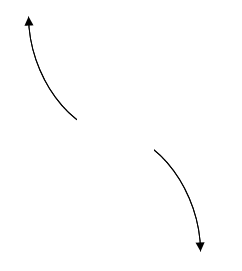
\includegraphics[width = 0.3\textwidth]{../Figures/polyEndBehaviorCopyAB.png}\item 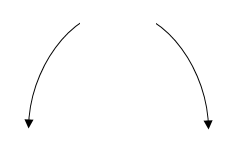
\includegraphics[width = 0.3\textwidth]{../Figures/polyEndBehaviorCopyBB.png}\item 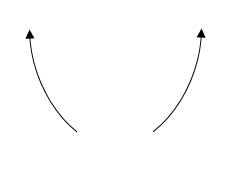
\includegraphics[width = 0.3\textwidth]{../Figures/polyEndBehaviorCopyCB.png}\item 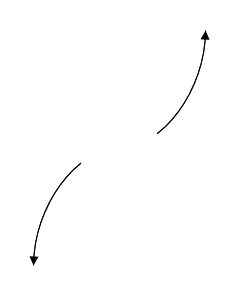
\includegraphics[width = 0.3\textwidth]{../Figures/polyEndBehaviorCopyDB.png}\end{multicols}\item None of the above.
\end{enumerate} }
\litem{
Describe the zero behavior of the zero $x = 5$ of the polynomial below.\[ f(x) = -6(x + 7)^{10}(x - 7)^{8}(x + 5)^{12}(x - 5)^{9} \]\begin{enumerate}[label=\Alph*.]
\begin{multicols}{2}\item 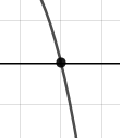
\includegraphics[width = 0.3\textwidth]{../Figures/polyZeroBehaviorAB.png}\item 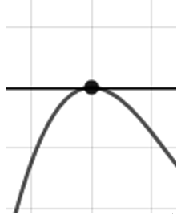
\includegraphics[width = 0.3\textwidth]{../Figures/polyZeroBehaviorBB.png}\item 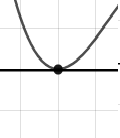
\includegraphics[width = 0.3\textwidth]{../Figures/polyZeroBehaviorCB.png}\item 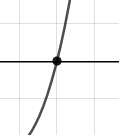
\includegraphics[width = 0.3\textwidth]{../Figures/polyZeroBehaviorDB.png}\end{multicols}\item None of the above.
\end{enumerate} }
\litem{
Construct the lowest-degree polynomial given the zeros below. Then, choose the intervals that contain the coefficients of the polynomial in the form $ax^3+bx^2+cx+d$.\[ \frac{-7}{5}, -4, \text{ and } \frac{-6}{5} \]\begin{enumerate}[label=\Alph*.]
\item \( a \in [24, 27], b \in [159, 167], c \in [296, 309], \text{ and } d \in [166, 170] \)
\item \( a \in [24, 27], b \in [159, 167], c \in [296, 309], \text{ and } d \in [-168, -161] \)
\item \( a \in [24, 27], b \in [-109, -104], c \in [-28, -20], \text{ and } d \in [166, 170] \)
\item \( a \in [24, 27], b \in [90, 102], c \in [-63, -56], \text{ and } d \in [-168, -161] \)
\item \( a \in [24, 27], b \in [-166, -163], c \in [296, 309], \text{ and } d \in [-168, -161] \)

\end{enumerate} }
\litem{
Construct the lowest-degree polynomial given the zeros below. Then, choose the intervals that contain the coefficients of the polynomial in the form $ax^3+bx^2+cx+d$.\[ \frac{5}{2}, \frac{-7}{5}, \text{ and } -5 \]\begin{enumerate}[label=\Alph*.]
\item \( a \in [9, 12], b \in [38, 45], c \in [-91, -85], \text{ and } d \in [171, 181] \)
\item \( a \in [9, 12], b \in [-45, -32], c \in [-91, -85], \text{ and } d \in [171, 181] \)
\item \( a \in [9, 12], b \in [55, 66], c \in [17, 22], \text{ and } d \in [-178, -168] \)
\item \( a \in [9, 12], b \in [38, 45], c \in [-91, -85], \text{ and } d \in [-178, -168] \)
\item \( a \in [9, 12], b \in [83, 95], c \in [227, 235], \text{ and } d \in [171, 181] \)

\end{enumerate} }
\litem{
Which of the following equations \textit{could} be of the graph presented below?
\begin{center}
    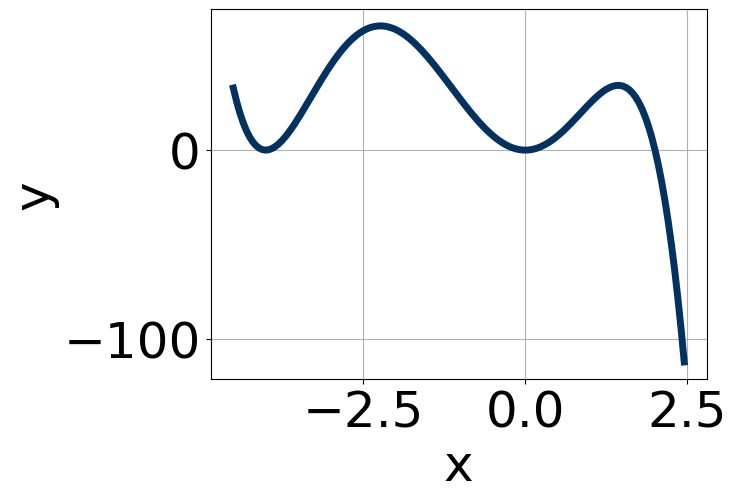
\includegraphics[width=0.5\textwidth]{../Figures/polyGraphToFunctionCopyB.png}
\end{center}
\begin{enumerate}[label=\Alph*.]
\item \( -2x^{4} (x - 2)^{8} (x + 1)^{4} \)
\item \( 17x^{6} (x - 2)^{4} (x + 1)^{9} \)
\item \( -12x^{9} (x - 2)^{10} (x + 1)^{7} \)
\item \( -17x^{4} (x - 2)^{6} (x + 1)^{9} \)
\item \( 11x^{6} (x - 2)^{4} (x + 1)^{8} \)

\end{enumerate} }
\litem{
Which of the following equations \textit{could} be of the graph presented below?
\begin{center}
    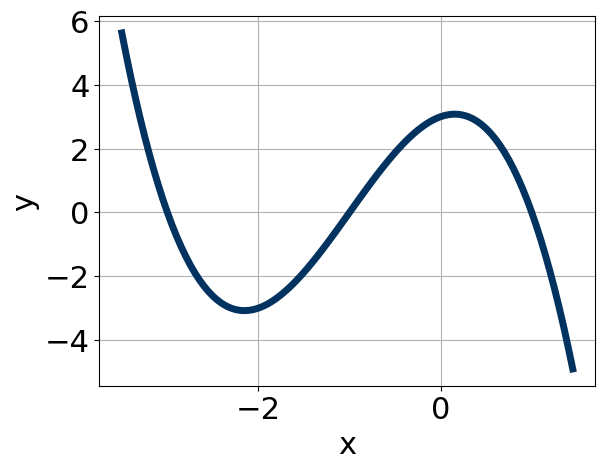
\includegraphics[width=0.5\textwidth]{../Figures/polyGraphToFunctionB.png}
\end{center}
\begin{enumerate}[label=\Alph*.]
\item \( -16x^{11} (x + 3)^{4} (x + 4)^{4} \)
\item \( -10x^{10} (x + 3)^{10} (x + 4)^{11} \)
\item \( 10x^{9} (x + 3)^{8} (x + 4)^{4} \)
\item \( 18x^{6} (x + 3)^{6} (x + 4)^{10} \)
\item \( -15x^{11} (x + 3)^{8} (x + 4)^{9} \)

\end{enumerate} }
\litem{
Describe the zero behavior of the zero $x = -2$ of the polynomial below.\[ f(x) = 9(x + 2)^{9}(x - 2)^{14}(x + 7)^{4}(x - 7)^{8} \]\begin{enumerate}[label=\Alph*.]
\begin{multicols}{2}\item 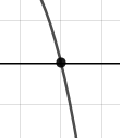
\includegraphics[width = 0.3\textwidth]{../Figures/polyZeroBehaviorCopyAB.png}\item 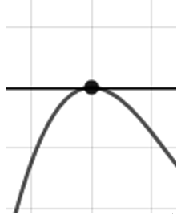
\includegraphics[width = 0.3\textwidth]{../Figures/polyZeroBehaviorCopyBB.png}\item 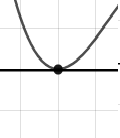
\includegraphics[width = 0.3\textwidth]{../Figures/polyZeroBehaviorCopyCB.png}\item 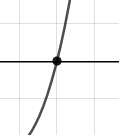
\includegraphics[width = 0.3\textwidth]{../Figures/polyZeroBehaviorCopyDB.png}\end{multicols}\item None of the above.
\end{enumerate} }
\litem{
Construct the lowest-degree polynomial given the zeros below. Then, choose the intervals that contain the coefficients of the polynomial in the form $x^3+bx^2+cx+d$.\[ 4 + 2 i \text{ and } 3 \]\begin{enumerate}[label=\Alph*.]
\item \( b \in [-3, 2], c \in [-8.19, -6.43], \text{ and } d \in [12, 18] \)
\item \( b \in [-18, -8], c \in [42.96, 45.21], \text{ and } d \in [-60, -55] \)
\item \( b \in [10, 12], c \in [42.96, 45.21], \text{ and } d \in [53, 64] \)
\item \( b \in [-3, 2], c \in [-5.57, -3.76], \text{ and } d \in [-2, 10] \)
\item \( \text{None of the above.} \)

\end{enumerate} }
\litem{
Describe the end behavior of the polynomial below.\[ f(x) = -4(x + 4)^{5}(x - 4)^{6}(x - 5)^{2}(x + 5)^{2} \]\begin{enumerate}[label=\Alph*.]
\begin{multicols}{2}\item 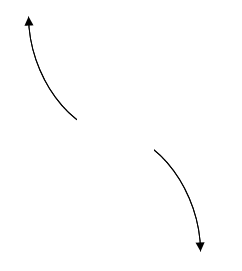
\includegraphics[width = 0.3\textwidth]{../Figures/polyEndBehaviorAB.png}\item 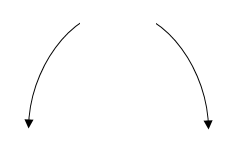
\includegraphics[width = 0.3\textwidth]{../Figures/polyEndBehaviorBB.png}\item 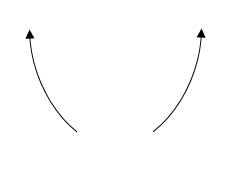
\includegraphics[width = 0.3\textwidth]{../Figures/polyEndBehaviorCB.png}\item 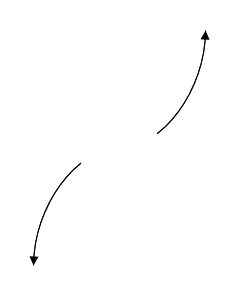
\includegraphics[width = 0.3\textwidth]{../Figures/polyEndBehaviorDB.png}\end{multicols}\item None of the above.
\end{enumerate} }
\end{enumerate}

\end{document}